\definecolor{tendonblue}{HTML}{1F4E99}

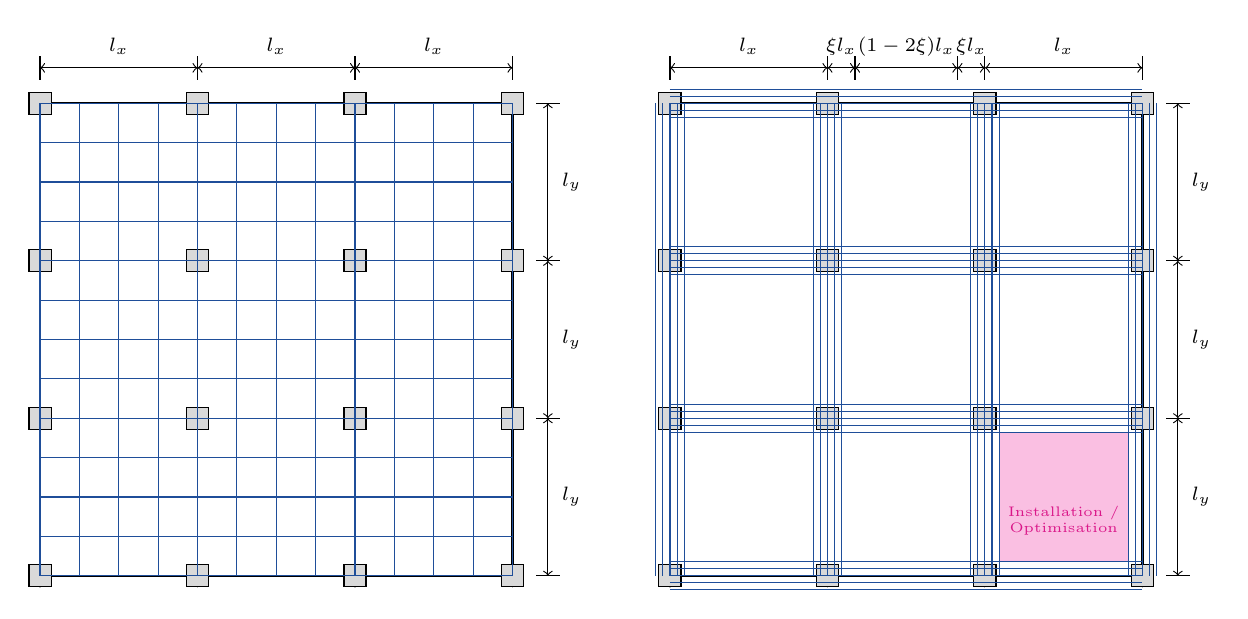
\begin{tikzpicture}[
    slab/.style={black, thick},
    tendon/.style={tendonblue, thin},
    gridline/.style={gray!45, dashed, thin},
    support/.style={draw, fill=gray!30, minimum size=0.28cm, inner sep=0pt},
    dim/.style={<->, thin},
    tick/.style={thin},
    txt/.style={font=\scriptsize},
    subtit/.style={font=\scriptsize\bfseries},
    note/.style={font=\scriptsize, align=center}
]

% Dimensions
\def\W{6.0}
\def\H{6.0}
\def\bayX{2.0}
\def\bayY{2.0}
\def\xA{0}
\def\xB{8.0}
\def\y{0}

% ============================================================
% (a) Distributed layout
% ============================================================

% Slab outline
\draw[slab] (\xA,\y) rectangle ++(\W,\H);

% Column grid lines
\foreach \xx in {0,2,4,6} {
    \draw[gridline] (\xA+\xx,\y-0.15) -- (\xA+\xx,\y+\H+0.15);
}
\foreach \yy in {0,2,4,6} {
    \draw[gridline] (\xA-0.15,\y+\yy) -- (\xA+\W+0.15,\y+\yy);
}

% Supports
\foreach \xx in {0,2,4,6} {
    \foreach \yy in {0,2,4,6} {
        \node[support] at (\xA+\xx,\y+\yy) {};
    }
}

% Distributed tendons aligned with column grid and extending to slab edges
\foreach \xx in {0,0.5,1.0,1.5,2.0,2.5,3.0,3.5,4.0,4.5,5.0,5.5,6.0} {
    \draw[tendon] (\xA+\xx,\y) -- (\xA+\xx,\y+\H);
}
\foreach \yy in {0,0.5,1.0,1.5,2.0,2.5,3.0,3.5,4.0,4.5,5.0,5.5,6.0} {
    \draw[tendon] (\xA,\y+\yy) -- (\xA+\W,\y+\yy);
}

% Dimensions x
\foreach \xx in {0,2,4} {
    \draw[dim] (\xA+\xx,\y+\H+0.45) -- (\xA+\xx+2,\y+\H+0.45);
    \draw[tick] (\xA+\xx,\y+\H+0.30) -- (\xA+\xx,\y+\H+0.60);
    \draw[tick] (\xA+\xx+2,\y+\H+0.30) -- (\xA+\xx+2,\y+\H+0.60);
    \node[txt] at (\xA+\xx+1,\y+\H+0.72) {$l_x$};
}

% Dimensions y
\foreach \yy in {0,2,4} {
    \draw[dim] (\xA+\W+0.45,\y+\yy) -- (\xA+\W+0.45,\y+\yy+2);
    \draw[tick] (\xA+\W+0.30,\y+\yy) -- (\xA+\W+0.60,\y+\yy);
    \draw[tick] (\xA+\W+0.30,\y+\yy+2) -- (\xA+\W+0.60,\y+\yy+2);
    \node[txt] at (\xA+\W+0.75,\y+\yy+1) {$l_y$};
}

% ============================================================
% (b) Banded layout
% ============================================================

% Slab outline
\draw[slab] (\xB,\y) rectangle ++(\W,\H);

% Column grid lines
\foreach \xx in {0,2,4,6} {
    \draw[gridline] (\xB+\xx,\y-0.15) -- (\xB+\xx,\y+\H+0.15);
}
\foreach \yy in {0,2,4,6} {
    \draw[gridline] (\xB-0.15,\y+\yy) -- (\xB+\W+0.15,\y+\yy);
}

% Supports
\foreach \xx in {0,2,4,6} {
    \foreach \yy in {0,2,4,6} {
        \node[support] at (\xB+\xx,\y+\yy) {};
    }
}

% Banded tendons along column strips, extending to slab edges
\foreach \yy in {0,2,4,6} {
    \foreach \dy in {-0.18,-0.09,0,0.09,0.18} {
        \draw[tendon] (\xB,\y+\yy+\dy) -- (\xB+\W,\y+\yy+\dy);
    }
}

\foreach \xx in {0,2,4,6} {
    \foreach \dx in {-0.18,-0.09,0,0.09,0.18} {
        \draw[tendon] (\xB+\xx+\dx,\y) -- (\xB+\xx+\dx,\y+\H);
    }
}

% Dimensions x with xi notation
\draw[dim] (\xB,\y+\H+0.45) -- (\xB+2,\y+\H+0.45);
\node[txt] at (\xB+1,\y+\H+0.72) {$l_x$};

\draw[dim] (\xB+2,\y+\H+0.45) -- (\xB+2.35,\y+\H+0.45);
\node[txt] at (\xB+2.175,\y+\H+0.72) {$\xi l_x$};

\draw[dim] (\xB+2.35,\y+\H+0.45) -- (\xB+3.65,\y+\H+0.45);
\node[txt] at (\xB+3.0,\y+\H+0.72) {$(1-2\xi)l_x$};

\draw[dim] (\xB+3.65,\y+\H+0.45) -- (\xB+4.0,\y+\H+0.45);
\node[txt] at (\xB+3.825,\y+\H+0.72) {$\xi l_x$};

\draw[dim] (\xB+4,\y+\H+0.45) -- (\xB+6,\y+\H+0.45);
\node[txt] at (\xB+5,\y+\H+0.72) {$l_x$};

\foreach \xx in {0,2,2.35,3.65,4,6} {
    \draw[tick] (\xB+\xx,\y+\H+0.30) -- (\xB+\xx,\y+\H+0.60);
}

% Dimensions y
\foreach \yy in {0,2,4} {
    \draw[dim] (\xB+\W+0.45,\y+\yy) -- (\xB+\W+0.45,\y+\yy+2);
    \draw[tick] (\xB+\W+0.30,\y+\yy) -- (\xB+\W+0.60,\y+\yy);
    \draw[tick] (\xB+\W+0.30,\y+\yy+2) -- (\xB+\W+0.60,\y+\yy+2);
    \node[txt] at (\xB+\W+0.75,\y+\yy+1) {$l_y$};
}

% Installation / optimisation field
\fill[magenta!25, draw=magenta!25, solid, thick]
    (\xB+4.2,\y+0.2) rectangle ++(1.6,1.6);
\node[note, magenta!90!black, font=\tiny] at (\xB+5,\y+0.70)
    {Installation /\\Optimisation};
\end{tikzpicture}%
}